\documentclass[12pt]{article}
\usepackage[utf8]{inputenc}

\usepackage{lmodern}

\usepackage{enumitem}
\usepackage[margin=2cm]{geometry}

\usepackage{amsmath, amsfonts, amssymb}
\usepackage{graphicx}
\usepackage{tikz}
\usepackage{pgfplots}
\usepackage{multicol}

\usepackage{comment}
\usepackage{url}
\usepackage{calc}
\usepackage{subcaption}

\usepackage{array}
\usepackage{blkarray,booktabs, bigstrut}

\pgfplotsset{compat=1.16}

% MATH commands
\newcommand{\ga}{\left\langle}
\newcommand{\da}{\right\rangle}
\newcommand{\oa}{\left\lbrace}
\newcommand{\fa}{\right\rbrace}
\newcommand{\oc}{\left[}
\newcommand{\fc}{\right]}
\newcommand{\op}{\left(}
\newcommand{\fp}{\right)}

\newcommand{\bi}{\mathbf{i}}
\newcommand{\bj}{\mathbf{j}}
\newcommand{\bk}{\mathbf{k}}
\newcommand{\bF}{\mathbf{F}}

\newcommand{\mR}{\mathbb{R}}

\newcommand{\ra}{\rightarrow}
\newcommand{\Ra}{\Rightarrow}

\newcommand{\sech}{\mathrm{sech}\,}
\newcommand{\csch}{\mathrm{csch}\,}
\newcommand{\curl}{\mathrm{curl}\,}
\newcommand{\dive}{\mathrm{div}\,}

\newcommand{\ve}{\varepsilon}
\newcommand{\spc}{\vspace*{0.5cm}}

\DeclareMathOperator{\Ran}{Ran}
\DeclareMathOperator{\Dom}{Dom}

\newcommand{\exo}[3]{\noindent\textcolor{red}{\fbox{\textbf{Section {#1} | Problem {#2} | {#3} points}}}\\}

\begin{document}
	\noindent \hrulefill \\
	MATH-302 \hfill Pierre-Olivier Paris{\'e}\\
	Homework 1 Solutions \hfill Fall 2022\\\vspace*{-0.7cm}
	
	\noindent\hrulefill
	
	\spc
	
	\exo{1.2}{1}{4}
	
	\begin{enumerate}[label=\alph*)]
	\item The highest derivative is $d^3y/dx^3$, and therefore the order of the ODE is $3$.
	\item The highest derivative is $y''$, and therefore the order of the ODE is $2$.
	\item The highest derivative is $y'$, and therefore the order of the ODE is $1$.
	\item The highest derivative is $y''$, and therefore the order of the ODE is $2$.
	\end{enumerate}
	
	\newpage
	
	\exo{1.2}{3b}{3}
	\\
	Integrate one time to get
		\begin{align*}
		y (x) = - \int x \sin x \, dx + c = \sin (x) - x \cos (x) + c 
		\end{align*}
	where $c$ is a constant.
	
	\vspace*{16pt}
		
	\exo{1.2}{3f}{3}
	\\
	Integrate a first time to get
		\begin{align*}
		y' (x) = x^2 - \cos x + e^x + c_1 
		\end{align*}
	where $c_1$ is a constant. Integrate a second time to get
		\begin{align*}
		y (x) = \frac{x^3}{3} - \sin x + e^x + c_1 x + c_2 
		\end{align*}
	where $c_2$ is a constant.
	
	\newpage
	
	\exo{1.2}{5a}{10}
	\\
	We see that
		\begin{align*}
		y(\pi / 4 ) = \frac{\pi \cos (\pi/4)}{4} = \frac{\pi}{4 \sqrt{2}} .
		\end{align*}
	The derivative is
		\begin{align*}
		y' (x) = \cos x - x \sin x  .
		\end{align*}
	Replacing $y$ in the left-hand side of the differential equation, we see that
		\begin{align*}
		\cos x - \frac{x \cos x \sin x}{\cos x} = \cos x  - x \sin x .
		\end{align*}
	Therefore, we see that $y' = \cos x - y \tan x$ and $y (\pi / 4) = \pi/ 4\sqrt{2}$.
	
	\vspace*{16pt}
	
	\exo{1.2}{5c}{10}
	\\
	We see that
		\begin{align*}
		y (0) = \tan \op \frac{0^2}{2} \fp = \frac{\sin (0)}{\cos (0)} = \frac{0}{1} = 0 .
		\end{align*}
	The derivative is
		\begin{align*}
		y' = x \sec^2 \op \frac{x^2}{2} \fp .
		\end{align*}
	Replacing $y$ in the left-hand side of the differential equation, we see that
		\begin{align*}
		 x (1 + y^2 ) = x \op 1 + \tan^2 \op \frac{x^2}{2} \fp \fp
		\end{align*}
	and, if you remembered some of your trig. identities, 
		\begin{align*}
		1 + \tan^2 (A) = \sec^2 (A)
		\end{align*}
	and therefore, with $A = x^2 /2$, we get
		\begin{align*}
		x (1 + y^2) = x \sec^2 \op \frac{x^2}{2} \fp .
		\end{align*}
	This is exactly the expression of $y'$ and so $y$ satisfies $y' = x (1 + y^2)$ and $y (0) = 0$.
	
	\newpage
	
	\exo{1.2}{9}{10}
	\\
	First, we remark that $e^x - 1 \geq 0$ when $x \geq 0$ because $e^x$ is increasing and $e^0 = 1$ and $1 - e^{-x} < 0$ when $x < 0$ because $e^{-x}$ is decreasing and $e^{0} = 1$. Therefore, the left-hand side of the differential equation is
		\begin{align*}
		|y| + 1 = e^x - 1 + 1 = e^x
		\end{align*}
	if $x \geq 0$ and
		\begin{align*}
		|y| + 1 = -(1 - e^{-x}) + 1 = e^{-x}
		\end{align*}
	if $x < 0$.
	
	For the left-hand side, when $x \geq 0$, then $y (x) = e^x - 1$ and therefore
		\begin{align*}
		y' (x) = e^x = |y| + 1 .
		\end{align*}
	When $x < 0$, then $y (x) = 1 - e^{-x}$ and therefore
		\begin{align*}
		y' (x) = e^{-x} = |y| + 1 .
		\end{align*}
	
	We just verified that for any $x$, $y' = |y| + 1$ and therefore $y$ satisfies the differential equation.
	
	\newpage
	
	\exo{1.3}{15}{10}
	\\
	\begin{itemize}
	\item \underline{Create a rectangular grid.}
	
	The rectangular grid is given: from $-2$ to $2$ in $x$ and from $0$ to $4$ in $y$. We place the nods at
		\begin{multicols}{2}
		\begin{itemize}
		\item $x_0 = -2$.
		\item $x_1 = 0$.
		\item $x_2 = 2$.
		\item $y_0 = 0$.
		\item $y_1 = 2$.
		\item $y_2 = 4$.
		\end{itemize}
		\end{multicols}
	This creates the following dotted grid:
		\begin{center}
		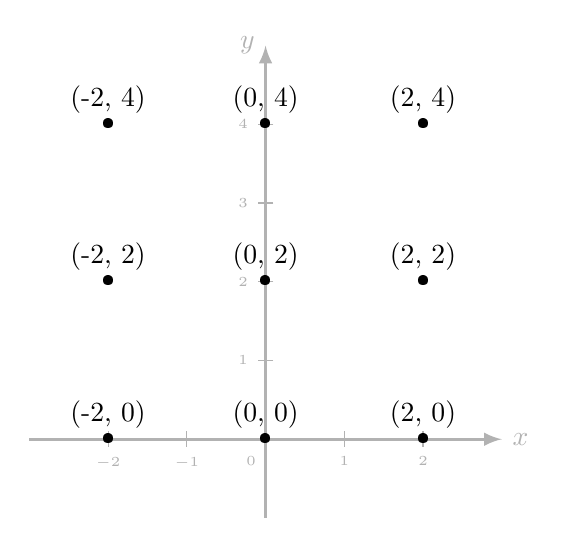
\begin{tikzpicture}
		\draw[->, >=latex, very thick, black!30] (-3, 0) -- (3, 0)node[right]{$x$};
		\draw[black!30] (-2, .1) -- (-2, -0.1)node[below]{{\tiny $-2$}};
		\draw[black!30] (-1, .1) -- (-1, -0.1)node[below]{{\tiny $-1$}};
		\draw[black!30] (0, .1) -- (0, -0.1)node[below left]{{\tiny $0$}};
		\draw[black!30] (1, .1) -- (1, -0.1)node[below]{{\tiny $1$}};
		\draw[black!30] (2, .1) -- (2, -0.1)node[below]{{\tiny $2$}};
		\draw[->, >=latex, very thick, black!30] (0, -1) -- (0, 5)node[left]{$y$};
		\draw[black!30] (.1, 1) -- (-0.1, 1)node[left]{{\tiny $1$}};
		\draw[black!30] (.1, 2) -- (-0.1, 2)node[left]{{\tiny $2$}};
		\draw[black!30] (.1, 3) -- (-0.1, 3)node[left]{{\tiny $3$}};
		\draw[black!30] (.1, 4) -- (-0.1, 4)node[left]{{\tiny $4$}};
		\draw[very thick] (-2, 0)node{\textbullet};
		\draw[very thick] (-2, 0)node[above]{(-2, 0)};
		\draw[very thick] (-2, 2)node{\textbullet};
		\draw[very thick] (-2, 2)node[above]{(-2, 2)};
		\draw[very thick] (-2, 4)node{\textbullet};
		\draw[very thick] (-2, 4)node[above]{(-2, 4)};
		\draw[very thick] (0, 0)node{\textbullet};
		\draw[very thick] (0, 0)node[above]{(0, 0)};
		\draw[very thick] (0, 2)node{\textbullet};
		\draw[very thick] (0, 2)node[above]{(0, 2)};
		\draw[very thick] (0, 4)node{\textbullet};
		\draw[very thick] (0, 4)node[above]{(0, 4)};
		\draw[very thick] (2, 0)node{\textbullet};
		\draw[very thick] (2, 0)node[above]{(2, 0)};
		\draw[very thick] (2, 2)node{\textbullet};
		\draw[very thick] (2, 2)node[above]{(2, 2)};
		\draw[very thick] (2, 4)node{\textbullet};
		\draw[very thick] (2, 4)node[above]{(2, 4)};
		\end{tikzpicture}
		\end{center}
		
	\item \underline{Find the slopes at each point of the grid.}
		\begin{multicols}{3}
		\begin{itemize}
		\item $(-2, 0)$: $y' = -6$
		\item $(-2, 2)$: $y' = -4$
		\item $(-2, 4)$: $y' = -2$
		\item $(0, 0)$: $y' = 0$
		\item $(0, 2)$: $y' = 2$
		\item $(0, 4)$: $y' = 4$
		\item $(2, 0)$: $y' = 6$
		\item $(2, 2)$: $y' = 8$
		\item $(2, 4)$: $y' = 10$
		\end{itemize}
		\end{multicols}
		
	\item \underline{Draw the actual direction field.} (All vectors are normalized)
	\begin{multicols}{2}
	\begin{center}
		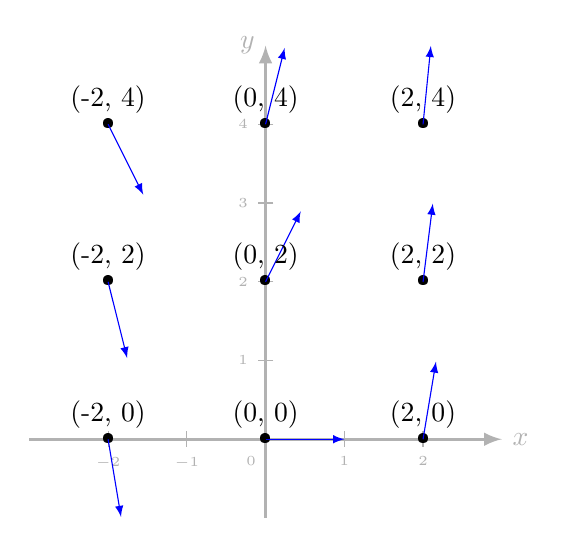
\begin{tikzpicture}
		\draw[->, >=latex, very thick, black!30] (-3, 0) -- (3, 0)node[right]{$x$};
		\draw[black!30] (-2, .1) -- (-2, -0.1)node[below]{{\tiny $-2$}};
		\draw[black!30] (-1, .1) -- (-1, -0.1)node[below]{{\tiny $-1$}};
		\draw[black!30] (0, .1) -- (0, -0.1)node[below left]{{\tiny $0$}};
		\draw[black!30] (1, .1) -- (1, -0.1)node[below]{{\tiny $1$}};
		\draw[black!30] (2, .1) -- (2, -0.1)node[below]{{\tiny $2$}};
		\draw[->, >=latex, very thick, black!30] (0, -1) -- (0, 5)node[left]{$y$};
		\draw[black!30] (.1, 1) -- (-0.1, 1)node[left]{{\tiny $1$}};
		\draw[black!30] (.1, 2) -- (-0.1, 2)node[left]{{\tiny $2$}};
		\draw[black!30] (.1, 3) -- (-0.1, 3)node[left]{{\tiny $3$}};
		\draw[black!30] (.1, 4) -- (-0.1, 4)node[left]{{\tiny $4$}};
		\draw[very thick] (-2, 0)node{\textbullet};
		\draw[blue, ->, >=latex] (-2, 0) -- ({-2 + cos(-80.54)}, {sin(-80.54)});
		\draw[very thick] (-2, 0)node[above]{(-2, 0)};
		\draw[very thick] (-2, 2)node{\textbullet};
		\draw[blue, ->, >=latex] (-2, 2) -- ({-2 + cos(-75.96)} , {2 + sin(-75.96)});
		\draw[very thick] (-2, 2)node[above]{(-2, 2)};
		\draw[very thick] (-2, 4)node{\textbullet};
		\draw[blue, ->, >=latex] (-2, 4) -- ({-2 + cos(-63.43)}, {4-sin(63.43)});
		\draw[very thick] (-2, 4)node[above]{(-2, 4)};
		\draw[very thick] (0, 0)node{\textbullet};
		\draw[blue, ->, >=latex] (0, 0) -- (1, 0);
		\draw[very thick] (0, 0)node[above]{(0, 0)};
		\draw[very thick] (0, 2)node{\textbullet};
		\draw[blue, ->, >=latex] (0, 2) -- ({cos(63.43)}, {2 + sin(63.43)});
		\draw[very thick] (0, 2)node[above]{(0, 2)};
		\draw[very thick] (0, 4)node{\textbullet};
		\draw[blue, ->, >=latex] (0, 4) -- ({cos(75.96)}, {4 + sin(75.96)});
		\draw[very thick] (0, 4)node[above]{(0, 4)};
		\draw[very thick] (2, 0)node{\textbullet};
		\draw[blue, ->, >=latex] (2, 0) -- ({2 + cos(80.54)}, {sin(80.54)});
		\draw[very thick] (2, 0)node[above]{(2, 0)};
		\draw[very thick] (2, 2)node{\textbullet};
		\draw[blue, ->, >=latex] (2, 2) -- ({2 + cos(82.87)}, {2 + sin(82.87)});
		\draw[very thick] (2, 2)node[above]{(2, 2)};
		\draw[very thick] (2, 4)node{\textbullet};
		\draw[blue, ->, >=latex] (2, 4) -- ({2 + cos(84.29)}, {4 + sin(84.29)});
		\draw[very thick] (2, 4)node[above]{(2, 4)};
		\end{tikzpicture}
		\end{center}
		
	\begin{itemize}
		\item $(-2, 0)$: $y' = -6$, $\measuredangle = -80.54^\circ$.
		\item $(-2, 2)$: $y' = -4$, $\measuredangle = -75.96^\circ$. 
		\item $(-2, 4)$: $y' = -2$, $\measuredangle = -63.43$.
		\item $(0, 0)$: $y' = 0$, $\measuredangle = 0^{\circ}$.
		\item $(0, 2)$: $y' = 2$, $\measuredangle = 63.43^\circ$.
		\item $(0, 4)$: $y' = 4$, $\measuredangle = 75.96^\circ$.
		\item $(2, 0)$: $y' = 6$, $\measuredangle = 80.54^\circ$.
		\item $(2, 2)$: $y' = 8$, $\measuredangle = 82.87^\circ$.
		\item $(2, 4)$: $y' = 10$, $\measuredangle = 84.29^\circ$.
		\end{itemize}
	\end{multicols}
	\end{itemize}
	
	\newpage
	
	Using Python, you would get (all vectors are normalized)
	
	\vspace*{16pt}
	
		\begin{minipage}{0.5\textwidth}
		\centering
		\includegraphics[scale=0.5]{exo15-sec1_3.png}
		With a $3 \times 3$ grid
		\end{minipage}
		\begin{minipage}{0.5\textwidth}
		\centering
		\includegraphics[scale=0.5]{exo15-sec1_3-more.png}
		With a $26 \times 26$ grid
		\end{minipage}
		
	\vfill
	
	\hfill \textcolor{red}{\textsc{Total (Points): 50.}}
	
\end{document}